%% Normalidade Contextual em APIs -- versão final (v9): regimes normais por tipo de dia x hora; decisão na hora anterior ao registro; limite no percentil 97
%% Classe acmart (sigconf), compatível com Overleaf (pdfLaTeX, XeLaTeX ou LuaLaTeX).
\documentclass[sigconf,nonacm]{acmart}

\usepackage[brazilian]{babel}
\usepackage{booktabs}
\usepackage{amsmath}
\usepackage{xspace}
\usepackage{fancyvrb}

\citestyle{acmauthoryear}
\settopmatter{printacmref=false, printfolios=true}
\renewcommand{\keywordsname}{Palavras-chave}
\setlength{\emergencystretch}{1.5em}

\newcommand{\Normal}{\textsc{Normal}\xspace}
\newcommand{\Residual}{\textsc{Residual}\xspace}

\begin{document}

\title{Normalidade Contextual em APIs: Caracterização de Regimes a partir de Access Logs para Apoio à Análise de Incidentes}

\author{Diego Paz Casagrande}
\affiliation{%
  \institution{Universidade de Brasília}
  \city{Brasília}
  \state{DF}
  \country{Brasil}}

\renewcommand{\shortauthors}{D. P. Casagrande}

\begin{abstract}
Quando um incidente é aberto, uma das primeiras perguntas do operador é se as APIs envolvidas estão operando normalmente e, se não estão, qual indicador saiu do padrão. A resposta não é trivial, porque uma API tem vários comportamentos normais, que variam legitimamente com o horário, o calendário e os processamentos em lote. Este trabalho investiga se \emph{API Access Logs} (AALs) agregados por minuto permitem caracterizar esses múltiplos regimes normais de cada endpoint e responder, no instante do registro do incidente, se o endpoint está dentro do regime normal esperado para aquele tipo de dia e hora (\Normal) ou fora dele (\Residual); qual indicador é responsável: erros de negócio (4xx), erros de sistema (5xx) ou latência; e desde quando. Seguindo o CRISP-DM, propõe-se um perfil de normalidade contextual por endpoint, com 48 regimes normais de referência (dia útil e não útil $\times$ 24 horas), cada um com mediana e MAD próprias, e um limite para cada indicador no percentil 97 dos seus desvios, calibrado por validação cruzada. A decisão compara a hora anterior ao registro com o regime do seu contexto, e uma expansão retroativa a partir do registro, em faixas de 15~min a 4~h, estima o início do desvio. Em 5,6 milhões de registros de 12 endpoints de produção no período de maio a setembro de 2026, testes estatísticos confirmaram regimes ligados à hora do dia em todos os recursos. Em 12.157 consultas simuladas em agosto e setembro, o método classificou corretamente 92,5\% dos controles como \Normal e sinalizou 48,7\% dos incidentes, apontando o indicador correto em 93,5\% deles; o início real ficou dentro da zona estimada em 89,4\%. A detecção foi alta para erros de sistema (até 89\%) e para degradações grandes de latência (83\% com 10 vezes), e baixa para erros de negócio. O perfil contextual superou um perfil sem contexto e empatou com a comparação com a semana anterior; seu maior valor está na explicação entregue ao operador.
\end{abstract}

\keywords{Mineração de Dados; API Access Log; Normalidade Contextual; Análise de Incidentes; CRISP-DM; Regimes Operacionais.}

\maketitle

%% =====================================================================
\section{Introdução}

A arquitetura dos sistemas modernos consolidou o uso de APIs (\emph{Application Programming Interfaces}) como mecanismo fundamental de integração em sistemas distribuídos. Em ambientes corporativos de grande porte, as APIs medeiam desde requisições de clientes externos até transações entre sistemas legados e modernos. No Banco do Brasil, cerca de 30 mil APIs são executadas diariamente, conectando soluções de negócio que combinam plataformas em nuvem e \emph{mainframe}.

\subsection{Contexto}

Requisições processadas por gateways de API geram registros com o instante da execução, o recurso acessado, o código de resposta, o tempo de processamento e o consumidor. Neste estudo, esses registros são denominados \emph{API Access Logs} (AALs), o registro gerado pelo gateway para as requisições processadas, distinto do \emph{execution log} e do log de aplicação. Os AALs estão disponíveis de forma padronizada para um conjunto amplo de APIs, sem instrumentação específica no código.

O comportamento operacional de uma API não é necessariamente estacionário. Volume, latência e proporção de erros variam com o horário, o dia da semana, os processamentos em lote e as janelas de manutenção. Uma taxa de erros elevada pode ser normal na virada do dia, assim como latência maior pode indicar degradação ou apenas um aumento esperado de volume de requisições; uma queda abrupta de tráfego pode indicar indisponibilidade ou o fim de um período de atendimento. Uma mesma API tem, portanto, vários comportamentos normais, cada um associado a um contexto de calendário e horário.

\subsection{Problema}
Quando um incidente é registrado, o operador precisa contextualizar semanticamente a situação e responder, para cada API envolvida: \emph{o período anterior ao registro estava dentro do comportamento normal esperado para aquele momento?} Se não estava, também importa saber quais métricas desviaram: erros de negócio (faixa 4xx), erros de sistema (faixa 5xx) ou latência; e desde quando o desvio acontece. Como informação complementar, interessa saber se o impacto é generalizado ou concentrado em uma aplicação cliente específica com volume suficiente para alterar o estado da API; um erro espalhado entre todos os consumidores sugere um problema no provedor.

Hoje essa resposta depende de consultar várias ferramentas e de conhecer o comportamento típico de cada API e endpoint~\citep{zhang2025isre}. Abordagens com limites fixos ou com um único perfil de normalidade não distinguem a variação legítima, como um lote à meia-noite ou o volume menor no domingo, de um desvio real.

Do ponto de vista de mineração de dados, o problema consiste em: (1) caracterizar os regimes normais de cada recurso a partir de AALs agregados em janelas; (2) classificar o período imediatamente anterior ao registro de um incidente em dois estados: \Normal (dentro de algum regime normal esperado para aquele contexto) ou \Residual (todo o resto); e (3) quando \Residual, identificar qual parâmetro desviou, sendo este o indicador responsável, e desde quando.

\subsection{Motivação}
Este trabalho complementa um projeto de mestrado sobre sistemas multiagente para apoio ao atendimento de incidentes. A literatura recente mostra agentes especializados em diferentes fontes de dados, coordenados para triagem e análise~\citep{yu2025triangle,luo2025opsagent,zhang2025isre}. Um desses agentes precisa de uma fonte confiável e explicável sobre o comportamento das APIs. O foco não é monitoração em tempo real nem a identificação da causa raiz, mas a \emph{informação de contexto no instante do incidente}: dizer se cada endpoint está em regime normal e, se não, qual indicador está impactado e desde quando. Essa informação abastece o operador por meio de um agente especialista e colabora para a análise do ocorrido, entregando um contexto semântico embasado nas atividades da mineração de dados, economizando recursos computacionais e evitando alucinações no agente, dada a quantidade de informações necessárias à análise.

\subsection{Objetivos}
\textbf{Objetivo geral:} caracterizar os regimes normais de cada endpoint da API a partir de Access Logs agregados por minuto e, no instante do registro de um incidente, informar se o endpoint está em regime normal e, se não, qual indicador foi impactado e desde quando.

\textbf{Objetivos específicos:}
\begin{itemize}
  \item Verificar se cada endpoint apresenta vários regimes normais ligados ao contexto (hora e tipo de dia).
  \item Construir um perfil de normalidade por endpoint e contexto e uma regra de decisão \Normal ou \Residual explicável.
  \item Identificar o indicador responsável (4xx, 5xx, latência) e estimar o início do desvio.
  \item Avaliar o método em cenários de incidente simulados em dois meses e compará-lo a baselines simples.
  \item Avaliar quanto histórico o perfil precisa (3 meses ou 1 mês).
  \item Disponibilizar a informação em formato estruturado para um agente ou operador.
\end{itemize}

\subsection{Questões de pesquisa}
\begin{itemize}
  \item \textbf{RQ1.} AALs agregados permitem caracterizar os regimes normais de cada recurso e decidir, no instante do registro, se o recurso está em regime normal?
  \item \textbf{RQ2.} Quando o recurso não está em regime normal, o método identifica corretamente o indicador responsável (4xx, 5xx, latência) e o início do desvio?
  \item \textbf{RQ3.} Um histórico mais longo (3 meses) produz um perfil melhor do que o histórico recente (1 mês)?
\end{itemize}

\subsection{Contribuições e organização}
As contribuições são: (i) a caracterização empírica dos regimes de 12 recursos de API de produção ao longo de cinco meses; (ii) um método simples e explicável, sem rótulos, que decide o estado de um recurso no instante do registro e aponta o indicador impactado; (iii) uma estimativa de início por expansão retroativa; (iv) um protocolo de avaliação com cenários de incidente simulados em dois meses; e (v) uma comparação entre históricos de 3 meses e de 1 mês. A Seção~\ref{sec:correlatos} discute os trabalhos correlatos; a Seção~\ref{sec:metodologia}, a metodologia; a Seção~\ref{sec:resultados}, os resultados; a Seção~\ref{sec:discussao}, a discussão; a Seção~\ref{sec:ameacas}, as ameaças à validade; e a Seção~\ref{sec:conclusao} conclui.

%% =====================================================================
\section{Trabalhos correlatos}\label{sec:correlatos}

A literatura relacionada é organizada em quatro frentes e avaliada segundo quatro critérios que decorrem do problema tratado aqui: (i) a fonte de dados exigida; (ii) o tratamento dado à normalidade, isto é, se o comportamento esperado é único ou condicionado ao contexto; (iii) o tipo de saída produzida, escore ou explicação; e (iv) a necessidade de rótulos ou de instrumentação adicional. A Tabela~\ref{tab:correlatos} resume a comparação.

\begin{table*}[t]
  \caption{Comparação com os trabalhos correlatos segundo os quatro critérios.}
  \label{tab:correlatos}
  \small
  \begin{tabular}{p{0.17\textwidth}p{0.19\textwidth}p{0.17\textwidth}p{0.2\textwidth}p{0.18\textwidth}}
    \toprule
    Trabalho & Fonte de dados & Normalidade & Saída & Rótulos ou instrumentação \\
    \midrule
    DeepLog, LogAnomaly & sequências de log de sistema & única & escore ou rótulo binário & log de aplicação com \emph{templates} \\
    SPOT/DSPOT & série temporal univariada & adaptada ao longo do tempo & limiar e alarme & --- \\
    USAD & séries multivariadas & única & escore & período de treino limpo \\
    \citet{wang2025crosssystem} & \emph{traces} & única por sistema & categoria da anomalia & \emph{traces}; exemplos rotulados \\
    DeepTraLog, GAMMA & \emph{traces}, logs e métricas & única & escore ou localização & instrumentação distribuída \\
    Triangle, OpsAgent, ISRE & múltiplas fontes do incidente & não modelada (consome evidências) & triagem ou diagnóstico & integração com as fontes \\
    \midrule
    \textbf{Este trabalho} & AAL agregado por minuto & família de regimes por contexto & estado, indicador e início, com explicação & nenhum além do AAL; sem rótulos \\
    \bottomrule
  \end{tabular}
\end{table*}

\subsection{Análise e mineração de logs}
\citet{du2017deeplog} propuseram o DeepLog, que modela sequências de eventos de log com redes LSTM e sinaliza como anômala toda sequência pouco provável sob o modelo aprendido. \citet{meng2019loganomaly} estenderam essa linha com o LogAnomaly, combinando a informação semântica dos \emph{templates} com a detecção de anomalias sequenciais e quantitativas. Ambos sustentam a premissa que também adotamos: logs carregam informação suficiente para caracterizar comportamento, sem instrumentação dedicada.

As diferenças, porém, são decisivas para o problema aqui tratado. Primeiro, a unidade de análise é a sequência de eventos de log de sistema, que pressupõe \emph{templates} estáveis e acesso ao log de aplicação; o AAL é um agregado por minuto, sem ordem de eventos e sem texto a partir do qual extrair \emph{templates}. Segundo, e mais importante, a normalidade nesses modelos é única: aprende-se uma distribuição de sequências normais, e o que foge dela é anômalo. Um lote à meia-noite ou uma janela de manutenção produzem padrões legítimos que um modelo sem contexto tende a tratar como desvio, a menos que o horário entre implicitamente como atributo, o que os trabalhos não exploram. Terceiro, a saída é um escore ou um rótulo binário. Para o operador que acaba de abrir um incidente, saber que a sequência é improvável não responde qual indicador saiu do padrão nem desde quando.

\subsection{Normalidade e séries temporais}
\citet{siffer2017dspot} propuseram o SPOT e sua variante com \emph{drift}, o DSPOT, que calibram limiares a partir da cauda da distribuição usando Teoria de Valores Extremos, com adaptação a séries não estacionárias. É o trabalho mais próximo do nosso em espírito: ambos reconhecem que o limiar não pode ser fixo e o derivam da própria distribuição observada, sem rótulos. O DSPOT adapta o limiar \emph{ao longo do tempo}, seguindo a série; o perfil contextual a trata como função de variáveis conhecidas \emph{a priori}, hora e tipo de dia. A consequência prática é que a adaptação temporal absorve uma degradação lenta como se fosse o novo normal, ao passo que o condicionamento por contexto preserva a referência do mesmo horário em dias anteriores. Em compensação, o DSPOT não exige que os contextos relevantes sejam conhecidos de antemão, o que é uma vantagem em domínios onde a sazonalidade não é óbvia.

\citet{audibert2020usad} propuseram o USAD, baseado em autoencoders para séries multivariadas. O método é mais expressivo que o nosso e captura dependências entre indicadores. Há ainda a questão do treinamento, que pressupõe um período limpo de anomalias; em dados de produção sem histórico de incidentes rotulado, como os nossos, essa suposição não é verificável.

\citet{wang2025crosssystem} documentam a dificuldade de transferir modelos de detecção entre sistemas distintos, mesmo com meta-aprendizado. O achado é relevante como justificativa negativa para nossa escolha de ajustar um perfil por recurso: se a transferência entre sistemas é difícil, a transferência entre recursos de perfis de tráfego muito diferentes nos nossos dados dificilmente seria mais fácil. A contrapartida é que perfis por recurso não generalizam para recursos novos, que precisam acumular histórico antes de serem avaliados; nossos resultados em setembro, com recursos de histórico curto, mostram esse custo.

\subsection{Modelagem comportamental de microsserviços}
O DeepTraLog~\citep{zhang2022deeptralog} combina \emph{traces} e logs em um grafo de eventos e aprende, com redes neurais em grafos, a estrutura esperada de uma requisição; o GAMMA~\citep{somashekar2024gamma} localiza gargalos de desempenho explorando a topologia de dependências entre serviços. Ambos entregam algo que o presente trabalho não entrega: localização, isto é, a indicação de \emph{onde} na cadeia de chamadas o problema se manifesta.

Esse ganho tem um pré-requisito. Ambos pressupõem \emph{traces} distribuídos ou métricas de infraestrutura correlacionadas, que exigem instrumentação consistente em todos os serviços da cadeia. Em ambientes corporativos heterogêneos, que combinam plataformas em nuvem e sistemas legados, essa cobertura é desigual. O AAL tem a propriedade oposta: é pobre em estrutura, porque não enxerga além do \emph{gateway}, mas é uniformemente disponível. Os dois enfoques são, portanto, complementares, e não concorrentes.

\subsection{Incidentes e sistemas multiagente}
O Triangle~\citep{yu2025triangle} organiza múltiplos agentes para a triagem de incidentes; o OpsAgent~\citep{luo2025opsagent} e o trabalho de \citet{zhang2025isre} coordenam agentes especializados em diferentes fontes para análise de incidentes e determinação de causa raiz. Esses sistemas deslocam o problema. O desafio deixa de ser o algoritmo de detecção e passa a ser a qualidade e a legibilidade das evidências que cada agente consome.

É nesse ponto que a avaliação desses trabalhos deixa uma questão em aberto. A competência do sistema multiagente é medida de ponta a ponta (acurácia de triagem, acerto de causa raiz), sem que se isole a contribuição de cada fonte nem se caracterize seu regime de erro.

\subsection{Síntese e lacuna}
A comparação revela um padrão: os trabalhos que dispensam rótulos tratam a normalidade como única ou como algo que se adapta ao longo do tempo, mas não como uma família de regimes legítimos coexistentes; os que modelam comportamento com riqueza suficiente para distinguir situações dependem de fontes além do AAL; e os que produzem explicações acionáveis o fazem no nível do sistema de agentes, assumindo como dadas as evidências que recebem. Nenhum deles investiga, exclusivamente a partir do AAL, se um mesmo recurso apresenta vários regimes normais e se essa caracterização pode informar, no instante do registro de um incidente, o estado do recurso, o indicador impactado e o início do desvio.

%% =====================================================================
\section{Metodologia}\label{sec:metodologia}

O trabalho segue o CRISP-DM~\citep{wirth2000crispdm,chapman2000crispdm}. Cada fase foi implementada em um \emph{notebook} Jupyter com parâmetros explícitos e sementes fixas (Tabela~\ref{tab:fases}). A análise é sempre por endpoint, unidade executável dentro de um produto de API. Optou-se por seis técnicas de mineração de dados no total, todas disponíveis em bibliotecas Python de uso corrente, como pandas, SciPy e scikit-learn~\citep{pedregosa2011sklearn}.

\begin{table}[t]
  \caption{Fases do CRISP-DM, notebooks e técnicas. As fases se repetem porque
  o processo é iterativo; a ordem segue a dos notebooks.}
  \label{tab:fases}
  \small
  \begin{tabular}{p{0.2\columnwidth}p{0.7\columnwidth}}
    \toprule
    Fase & Notebook: conteúdo (técnica) \\
    \midrule
    Negócio, Dados & 01: problema, critérios de sucesso, qualidade e evolução mensal da base \\
    Preparação & 02: consolidação, indicadores por janela, p95 de latência (percentil) \\
    Dados, Modelagem & 03: regimes (Kruskal-Wallis com Bonferroni; k-means com silhouette) \\
    Modelagem & 04: perfil contextual (mediana/MAD); limite por indicador (percentil, validação cruzada), por mês de teste e histórico \\
    Preparação & 05: cenários de incidente (injeção de falhas) \\
    Avaliação & 06: estado, indicador, início (expansão retroativa); histórico; IC de Wilson, McNemar \\
    Implantação & 07: consulta estruturada para o agente \\
    \bottomrule
  \end{tabular}
\end{table}

\subsection{Entendimento do negócio}
A decisão apoiada é: \emph{no instante do registro do incidente, o recurso está em regime normal? Se não, qual indicador foi impactado (erros 4xx, erros 5xx, latência) e desde quando?} A abrangência (consumidor específico ou generalizado) é informação complementar. Os critérios de sucesso foram definidos antes da modelagem (Tabela~\ref{tab:criterios}). Como não havia histórico de incidentes, a avaliação usa cenários simulados com falhas injetadas.

\subsection{Entendimento dos dados}
A base contém AALs de produção de 12 endpoints de APIs distintas, identificados aqui por E01 a E12 (em ordem decrescente de volume em agosto). Cada registro é um agregado por minuto de data e hora da execução, endpoint, código de resposta HTTP e cliente, com o total de execuções no minuto e o tempo médio dessas execuções. Como a agregação temporal por minuto já está disponível neste formato, optou-se por não utilizar os registros por execução, o que não impede que o registro bruto seja agregado da mesma forma e usado como entrada deste processo. O identificador de cliente foi anonimizado por SHA-256 com semente, sem payloads nem dados pessoais. Os horários, em UTC, foram convertidos para o horário de Brasília (UTC$-3$) antes de qualquer corte temporal.

São 5.632.001 registros de 30/04/2026 21h a 20/09/2026 20h59 (horário de Brasília), com 1.976 clientes distintos. As respostas de sucesso (2xx) somam 87,6\% das transações; os erros de negócio (4xx), 12,1\%; e os erros de sistema (5xx), 0,21\%. A cobertura varia: sete recursos têm dados desde maio; o E04, desde 25/05; cinco (E02, E03, E06, E10, E11), apenas desde 16/07; e quatro (E02, E03, E06, E11) param em 03/09. O volume mediano por hora vai de 248 transações (E11) a 9.470 (E02). Esses números mostram a heterogeneidade da base entre endpoints.

\paragraph{Evolução mensal.} O comportamento muda ao longo dos meses. Entre maio e setembro, o volume médio diário cresce de 35\% a 60\% em vários recursos (E07, E08, E12), e a taxa de erros de negócio muda de patamar: no E02, passa de 32\% (julho) para 45\% (agosto) e 62\% (setembro); no E04, de 0,5\% (maio) para 13\% (agosto). Essa mudança motiva a questão RQ3.

\subsection{Preparação dos dados}
As chaves repetidas foram consolidadas (soma do volume e média de latência ponderada). Os registros foram agregados em janelas de 1~h (29.695 janelas recurso $\times$ hora), que formam a base do perfil de normalidade e da decisão no registro. Faixas menores que 1~h (15 e 30~min) são usadas apenas para estimar o início do desvio. A decisão usa quatro indicadores (Tabela~\ref{tab:atributos}). O \emph{contexto} de cada janela é o par (tipo de dia, hora), com tipo de dia \emph{útil} ou \emph{não útil} (sábado, domingo e feriados: 01/05, 04/06 e 07/09).

\paragraph{Latência p95.} Como não há latência por requisição, o p95 é o percentil 95 das latências médias por minuto $\times$ cliente das respostas 2xx, ponderado pelo número de execuções. É um p95 \emph{das médias}, não das requisições, e tende a subestimar a cauda real; mas é consistente entre períodos e sensível a degradações que atingem só parte dos minutos ou dos consumidores. Na mediana, ele é 1,42 vez a latência média.

\begin{table}[t]
  \caption{Indicadores usados na decisão e direção desfavorável.}
  \label{tab:atributos}
  \small
  \begin{tabular}{p{0.2\columnwidth}p{0.52\columnwidth}p{0.16\columnwidth}}
    \toprule
    Indicador & Definição & Direção \\
    \midrule
    volume & $\log(1+$transações$)$, na escala horária & alta e queda \\
    erros 4xx & transações 4xx / total (erros de negócio) & alta \\
    erros 5xx & transações 5xx / total (erros de sistema) & alta \\
    latência p95 & $\log(1+$p95 das médias por minuto$\times$cliente$)$ & alta \\
    \bottomrule
  \end{tabular}
\end{table}

\subsection{Modelagem}

\paragraph{Grupos de comportamento (descritivo).} O teste de Kruskal-Wallis~\citep{kruskal1952ranks}, com correção de Bonferroni~\citep{dunn1961multiple}, verifica se cada indicador muda entre as 24 horas dos dias úteis. Para cada recurso, o k-means~\citep{lloyd1982kmeans} agrupa as janelas de 1~h de maio a agosto usando apenas os indicadores padronizados e limitados aos percentis 1 e 99 do recurso (em um período de quatro meses, picos isolados formariam grupos próprios com menos de 0,5\% das horas). O número de grupos, $k\in[2,8]$, é escolhido pelo coeficiente de silhouette~\citep{rousseeuw1987silhouette}. O contexto não entra no agrupamento, para que a relação entre comportamento e contexto seja uma descoberta, e não um insumo; ele é usado depois, para nomear cada grupo (nível de volume, tipo de dia e horas em que predomina). O k-means é descritivo: mostra que os contextos se organizam em poucos comportamentos típicos, mas a decisão usa o regime de cada contexto.

\paragraph{Perfil de normalidade contextual.} Para o recurso $r$, contexto $c$ e indicador $a$, o perfil guarda a mediana histórica $m_a(r,c)$ e uma escala robusta de variação~\citep{leys2013mad}, calculadas nas janelas de 1~h do histórico:
\begin{equation}
  s_{a}(r,c)=\max\{1{,}4826\cdot\mathrm{MAD}_{a}(r,c),\ \varepsilon_a\},
\end{equation}
em que o fator 1,4826 torna o MAD comparável ao desvio-padrão e $\varepsilon_a$ é um piso que evita divisões por valores próximos de zero. Para um período $w$ do recurso $r$ no contexto $c$, o desvio de cada indicador é
\begin{equation}
  z_a(w)=\frac{x_a(w)-m_a(r,c)}{s_a(r,c)},
\end{equation}
isto é, quantas escalas de variação normal o indicador se afasta do esperado. Para o volume, tanto aumentos como quedas são desfavoráveis ($d_a=|z_a|$); para erros 4xx, erros 5xx e latência, apenas aumentos contam ($d_a=\max\{z_a,0\}$). Com dois tipos de dia e 24 horas, cada recurso tem assim 48 \emph{regimes normais} de referência, cada um com a sua mediana, escala e faixa p5--p95; o período é avaliado contra o regime do seu contexto.

\paragraph{Limite por indicador.} Os indicadores têm variabilidades muito diferentes; em alguns endpoints a taxa de 4xx tem picos reais frequentes. Um único limiar sobre o maior desvio seria dominado pelos indicadores mais ruidosos e esconderia desvios nos demais. Por isso, cada indicador tem um limite próprio no recurso, $L_{r,a}=\max\{3,\ Q_{0{,}97}(d_a)\}$: o percentil 97 dos seus desvios no histórico, calculados fora da amostra. O período é \Residual se algum indicador passa do seu limite ($d_a/L_{r,a}>1$); o \textbf{indicador responsável} é o que mais passou, em múltiplos do limite.

\paragraph{Histórico e calibração sem vazamento.} Para cada mês de teste (agosto; 1 a 20 de setembro), o perfil e os limites são ajustados só com dados anteriores, em dois históricos: \emph{3 meses} (principal; maio a julho para agosto e junho a agosto para setembro) e \emph{1 mês} (o mês anterior). Os desvios fora da amostra vêm de validação cruzada com quatro blocos contíguos de tempo dentro do histórico: o perfil é ajustado em três blocos e avalia o restante. Com essa regra, cerca de 9\% dos períodos do histórico ficam fora do regime normal do seu contexto.

\paragraph{Consulta no registro.} No instante $t$ do registro, o \emph{estado} do recurso é decidido sobre a hora anterior ao registro, $[t-60\,\text{min}, t)$, comparada ao perfil do seu contexto: o tipo de dia e a hora do ponto médio dessa janela. Se algum indicador passa do seu limite, o recurso está \Residual, e o indicador responsável é o que mais passou.

\paragraph{Início estimado (expansão retroativa).} Quando o recurso está \Residual, o método estima desde quando, olhando para trás a partir de $t$ em faixas disjuntas cada vez mais distantes: 0--15, 15--30 e 30--60~min e, depois, de hora em hora até 4~h. Essas faixas curtas servem \emph{apenas} para localizar o início; não entram na decisão do estado. A busca parte da faixa residual mais recente e para na primeira faixa \Normal; o início é estimado entre o começo da última faixa residual e o fim dessa faixa normal (``começou entre 30 e 120~min antes do registro''). Todas as faixas são comparadas ao mesmo perfil de 1~h: o volume é convertido para a escala horária, e as taxas e o p95 são usados diretamente. Como faixas curtas variam mais, cada tamanho de faixa recebe seus próprios limites, calibrados da mesma forma. Se nenhuma faixa curta sair do normal, o início fica indeterminado.

\paragraph{Abrangência (complementar).} Para erros 4xx ou 5xx, o desvio é atribuído a um \emph{consumidor específico} quando o cliente com mais erros concentra ao menos 80\% deles e essa fatia supera em pelo menos 20 pontos percentuais a sua fatia do volume; caso contrário, é \emph{generalizado}. Recursos com menos de três clientes ativos ficam indeterminados.

\subsection{Avaliação}

\paragraph{Cenários de incidente.} Cada cenário simula um incidente: uma degradação começa em $t_0$ e o incidente é registrado em $t=t_0+\Delta$, com atraso $\Delta\in\{15,30,60,120\}$~min. O instante de registro é sorteado dentro do mês de teste. Entram no teste de um mês os recursos com ao menos 28 dias de dados no mês anterior: 7 recursos em agosto e os 12 em setembro. As falhas (Tabela~\ref{tab:falhas}) são aplicadas nos registros por minuto $\times$ cliente e depois reagregadas, para que os indicadores e a abrangência reajam como numa falha real. Foram gerados 5 cenários por recurso $\times$ mês $\times$ motivo $\times$ intensidade $\times$ atraso (6.080 incidentes, dos quais 3 sem tráfego foram descartados) e 6.080 consultas de controle, em instantes sem falha injetada.

\begin{table}[t]
  \caption{Motivos injetados.}
  \label{tab:falhas}
  \small
  \begin{tabular}{p{0.26\columnwidth}p{0.64\columnwidth}}
    \toprule
    Motivo & Intensidade (baixa / média / alta / muito alta) \\
    \midrule
    4xx generalizado & 5\% / 15\% / 40\% das 2xx viram 400 \\
    4xx de 1 consumidor & 30\% / 60\% / 90\% das 2xx do consumidor viram 400 \\
    5xx generalizado & 5\% / 15\% / 40\% das 2xx viram 503 \\
    5xx de 1 consumidor & 30\% / 60\% / 90\% das 2xx do consumidor viram 503 \\
    Latência & tempo de execução $\times$1,5 / $\times$2,5 / $\times$4 / $\times$10 \\
    \bottomrule
  \end{tabular}
  \par\smallskip\footnotesize O consumidor afetado é sorteado com probabilidade proporcional ao seu volume.
\end{table}

\paragraph{Latência $\times$10.} Como a latência vem de médias por minuto, poucas requisições lentas elevam muito o valor. No histórico de maio a agosto, o p95 horário ultrapassou 10 vezes a mediana do seu contexto em 0,78\% das horas (percentil 99,9: 25 vezes; máximo: 68 vezes). Degradações de latência relevantes para um incidente tendem a ser desse tamanho, por isso a intensidade ``muito alta'' ($\times$10) foi incluída para a latência. As intensidades menores foram mantidas para mostrar o limite do método.

\paragraph{Métricas.} Para cada cenário, a consulta é feita no instante do registro, como descrito acima. As métricas são: \emph{sensibilidade} (incidentes com saída \Residual); \emph{especificidade} (controles com saída \Normal); \emph{acurácia do indicador} (indicador apontado igual ao do motivo injetado, entre os detectados); \emph{acerto do início} (início real dentro da zona estimada pela expansão retroativa); e \emph{acurácia da abrangência}. ``Média/alta'' refere-se às intensidades média e alta, sem a latência $\times$10, que é relatada à parte. As proporções têm intervalos de confiança de Wilson a 95\%~\citep{wilson1927probable}.

\paragraph{Baselines.} Os baselines avaliam se o perfil contextual agrega valor à decisão. O primeiro é o \emph{z-score global}, que usa a mesma lógica de mediana, MAD e limites por indicador, mas ignora hora e tipo de dia: cada endpoint tem uma única referência histórica para cada indicador. O segundo é a \emph{semana anterior}, que compara o período avaliado com o mesmo intervalo de tempo sete dias antes, explorando a periodicidade semanal sem construir um perfil estatístico mais amplo. Os três métodos usam o mesmo tratamento de limites e calibração, para que a comparação isole o efeito da estratégia de referência.

A comparação entre métodos usa o teste exato de McNemar~\citep{mcnemar1947note} sobre os acertos de estado nos mesmos cenários simulados. O teste considera apenas os casos em que os métodos divergem: aqueles em que o perfil contextual acerta e o baseline erra, e aqueles em que ocorre o contrário. Um valor $p$ pequeno indica evidência de diferença estatisticamente significativa entre os métodos. O mesmo teste compara os perfis ajustados com históricos de 3 meses e de 1 mês, pois ambos são aplicados aos mesmos cenários.

\paragraph{Experimentos.} \textbf{Exp.~1} caracteriza os regimes de cada recurso (Kruskal-Wallis e k-means). \textbf{Exp.~2} avalia o estado no registro: sensibilidade, especificidade e comparação com os baselines. \textbf{Exp.~3} avalia a consulta quando o recurso é \Residual: indicador responsável, início estimado pela expansão retroativa e abrangência. \textbf{Exp.~4} compara os históricos de 3 meses e de 1 mês.

%% =====================================================================
\section{Resultados}\label{sec:resultados}

\subsection{Exp.~1: regimes normais por recurso}

A Figura~\ref{fig:perfis} mostra perfis horários típicos: lote na virada do dia e às 18h dos dias úteis (E01), lote às 15--16h (E05), padrão comercial em dias úteis que desaparece nos dias não úteis (E02, E12). O mapa de calor (Figura~\ref{fig:mapa}) confirma que cada recurso tem sua própria assinatura horária de volume e de latência.

\begin{figure*}[t]
  \centering
  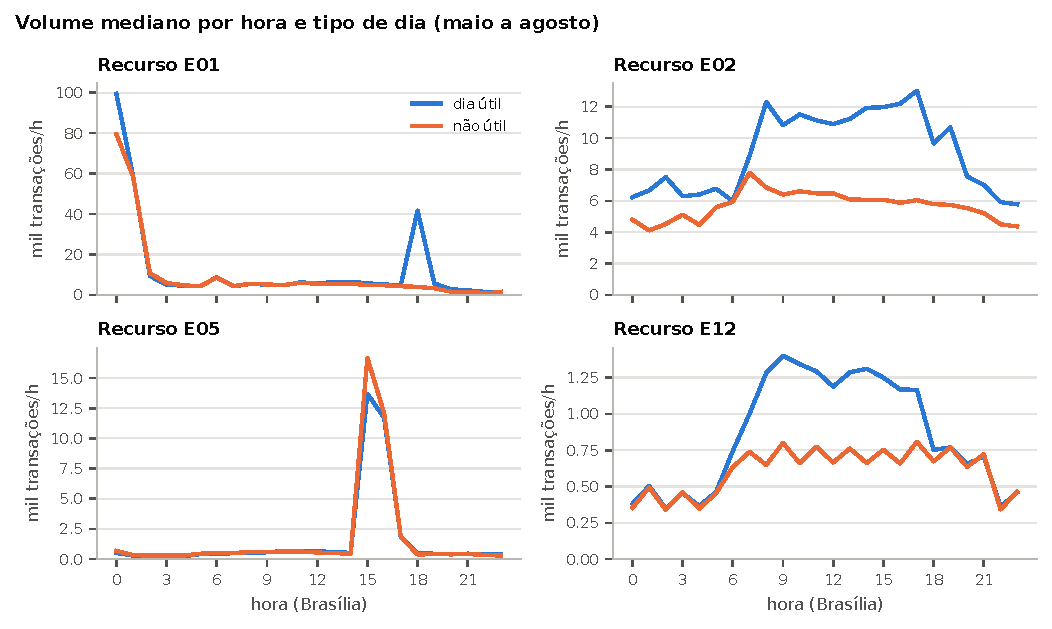
\includegraphics[width=0.9\textwidth]{figuras/fig_perfis_volume.pdf}
  \caption{Volume mediano por hora e tipo de dia (maio a agosto), em quatro recursos.}
  \label{fig:perfis}
\end{figure*}

\begin{figure*}[t]
  \centering
  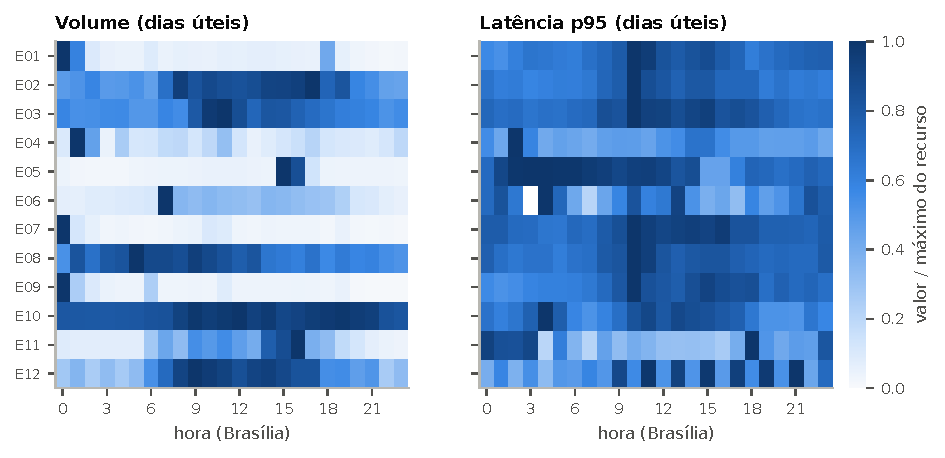
\includegraphics[width=0.85\textwidth]{figuras/fig_mapa_calor.pdf}
  \caption{Volume e latência p95 medianos por hora em dias úteis, normalizados pelo máximo de cada recurso.}
  \label{fig:mapa}
\end{figure*}

Nos dias úteis, 96\% dos testes de Kruskal-Wallis (recurso $\times$ indicador) foram significativos após Bonferroni. O efeito mediano ($\varepsilon^2$) foi grande para volume (0,40), erros 4xx (0,28) e latência p95 (0,25), e pequeno para erros 5xx (0,05), que em dias normais são raros. O comportamento normal de cada recurso depende, portanto, do horário, o que justifica um regime normal por contexto.

O k-means encontrou de 2 a 8 grupos de comportamento por recurso (mediana 3; silhouette médio 0,51; Tabela~\ref{tab:recursos}), e cada grupo ocupa um conjunto de contextos. A Figura~\ref{fig:regimes} ilustra o E02: um comportamento de volume alto das 8 às 19h dos dias úteis, um de volume médio no restante do tempo, um de volume baixo em dias não úteis e um comportamento à 0h com taxa de 5xx elevada. Esse último é \emph{normal} para aquele horário: é o tipo de variação legítima que um limite fixo trataria como falha, e que o regime do contexto ``dia útil, 0h'' acomoda com a sua própria faixa normal.

\begin{figure*}[t]
  \centering
  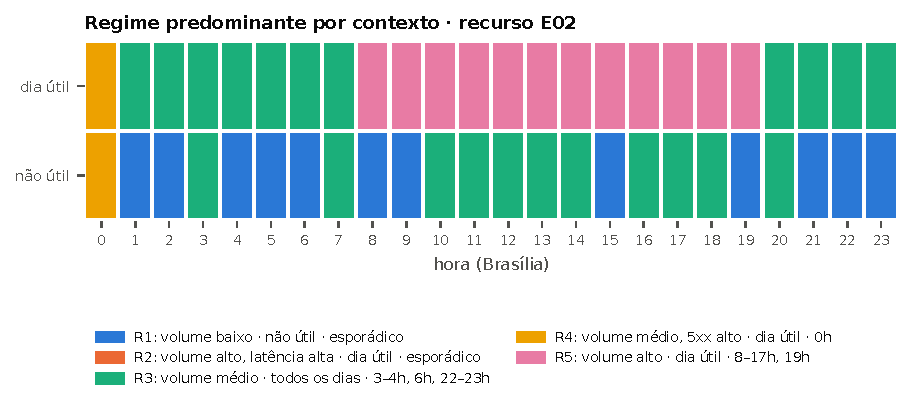
\includegraphics[width=0.85\textwidth]{figuras/fig_regimes_contexto.pdf}
  \caption{Comportamento predominante (k-means com os indicadores) por tipo de dia e hora no recurso E02.}
  \label{fig:regimes}
\end{figure*}

\begin{table*}[t]
  \caption{Resumo por recurso: participação no volume, clientes, transações medianas por hora, grupos de comportamento (Exp.~1), meses de teste e resultados da consulta no registro (Exp.~2 e 3, histórico de 3 meses).}
  \label{tab:recursos}
  \small
  \begin{tabular}{lrrrrrcrrrr}
    \toprule
    Recurso & Vol. (\%) & Clientes & Trans./h & Grupos ($k$) & Silhouette & Teste & Sensib. & Sensib. média/alta & Especif. & Acurácia indicador \\
    \midrule
    E01 & 47,3 & 38  & 5.120 & 3 & 0,36 & ago, set & 0,68 & 0,80 & 0,88 & 0,94 \\
    E02 & 11,9 & 555 & 9.470 & 5 & 0,55 & set & 0,14 & 0,21 & 0,98 & 0,91 \\
    E03 & 3,1  & 246 & 2.535 & 4 & 0,52 & set & 0,21 & 0,24 & 0,99 & 0,95 \\
    E04 & 4,9  & 24  & 925   & 2 & 0,54 & ago, set & 0,43 & 0,44 & 0,91 & 0,87 \\
    E05 & 6,0  & 19  & 483   & 2 & 0,78 & ago, set & 0,76 & 0,84 & 0,93 & 0,94 \\
    E06 & 2,4  & 787 & 1.583 & 2 & 0,64 & set & 0,07 & 0,06 & 0,98 & 0,78 \\
    E07 & 5,7  & 36  & 596   & 2 & 0,63 & ago, set & 0,47 & 0,51 & 0,92 & 0,93 \\
    E08 & 5,9  & 39  & 1.128 & 5 & 0,35 & ago, set & 0,53 & 0,61 & 0,95 & 0,97 \\
    E09 & 5,6  & 30  & 578   & 3 & 0,66 & ago, set & 0,69 & 0,77 & 0,87 & 0,95 \\
    E10 & 2,2  & 2   & 1.038 & 8 & 0,29 & set & 0,24 & 0,24 & 0,96 & 0,89 \\
    E11 & 1,9  & 625 & 248   & 3 & 0,55 & set & 0,26 & 0,29 & 0,99 & 0,94 \\
    E12 & 2,9  & 831 & 723   & 4 & 0,29 & ago, set & 0,61 & 0,69 & 0,88 & 0,93 \\
    \bottomrule
  \end{tabular}
\end{table*}

\subsection{Perfil de normalidade e limites}
Os limites por indicador (Figura~\ref{fig:limites}) variam de 3 a 51 em $z$. Limites altos revelam indicadores com picos reais frequentes no histórico: erros 4xx em E04 (51), E07 (31) e E01 (10); latência p95 em E02 (29) e E03 (14); e volume em E11 (21) e E09 (8). Nesses casos, só desvios grandes daquele indicador são marcados como \Residual. Os erros 5xx, raros em dias normais, ficam no limite mínimo de 3 em quase todos os recursos. No histórico de junho a agosto, fora da amostra, 8,7\% das janelas de 1~h ficaram fora do regime normal do seu contexto, com latência (590 janelas), volume (568), erros 4xx (505) e erros 5xx (158) como indicadores responsáveis. Os indicadores responsáveis estão, portanto, distribuídos de forma equilibrada: nenhum deles domina a decisão, que é o objetivo do limite por indicador.

\begin{figure}[t]
  \centering
  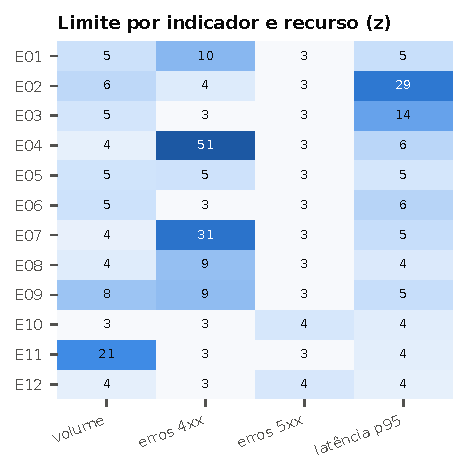
\includegraphics[width=0.75\columnwidth]{figuras/fig_limites.pdf}
  \caption{Limite de cada indicador por recurso ($z$, percentil 97 fora da amostra, mínimo 3) nas janelas de 1~h; histórico de junho a agosto.}
  \label{fig:limites}
\end{figure}

\subsection{Exp.~2: estado no instante do registro}
A Tabela~\ref{tab:metodos} e a Figura~\ref{fig:metodos} resumem a decisão sobre a hora anterior ao registro. O perfil contextual classificou corretamente 92,5\% dos controles como \Normal e sinalizou como \Residual 48,7\% dos incidentes (54,6\% nas intensidades média e alta). Nos acertos de estado, ele supera o z-score global (McNemar: $p=0{,}020$; 540 casos em que só o perfil acerta, contra 465) e empata com a semana anterior ($p=0{,}054$). O ganho sobre o z-score global vem da detecção (54,6\% contra 49,6\% nas intensidades média e alta), com especificidade menor (92,5\% contra 95,5\%): sem contexto, uma única referência por recurso precisa acomodar todos os horários, e só desvios grandes passam do limite.

\begin{table*}[t]
  \caption{Exp.~2: estado no registro (hora anterior) por método, em \% (IC de Wilson a 95\% entre colchetes). Histórico de 3 meses; 6.077 incidentes e 6.080 controles. $p$: McNemar dos acertos de estado contra o método proposto.}
  \label{tab:metodos}
  \small
  \begin{tabular}{lccccc}
    \toprule
    Método & Sensibilidade & Sensibilidade (média/alta) & Especificidade & Acurácia do indicador & $p$ \\
    \midrule
    \textbf{Perfil contextual (proposto)} & \textbf{48,7} [47,5; 50,0] & \textbf{54,6} [53,0; 56,1] & 92,5 [91,8; 93,2] & 93,5 & --- \\
    z-score global & 44,5 [43,2; 45,7] & 49,6 [48,0; 51,2] & 95,5 [95,0; 96,0] & 95,7 & 0,020 \\
    Semana anterior & 49,4 [48,1; 50,6] & 55,3 [53,7; 56,9] & 92,9 [92,3; 93,6] & 93,7 & 0,054 \\
    \bottomrule
  \end{tabular}
\end{table*}

\begin{figure*}[t]
  \centering
  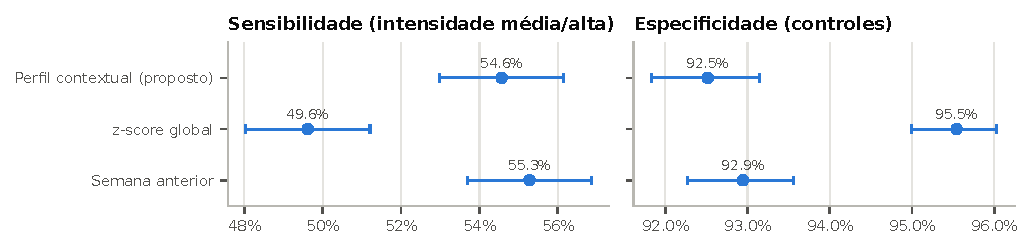
\includegraphics[width=0.85\textwidth]{figuras/fig_metodos.pdf}
  \caption{Sensibilidade (intensidades média e alta) e especificidade por método, com IC de Wilson a 95\%.}
  \label{fig:metodos}
\end{figure*}

\paragraph{Ponto de operação.} O limite de cada indicador é o seu percentil 97 no histórico, um meio-termo entre detectar mais e alarmar menos. A Figura~\ref{fig:curva} mostra a curva de operação do método: com metas mais conservadoras, de 1\%, 2\% e 5\% de alarmes no histórico, a especificidade sobe para 99,4\%, 98,4\% e 95,6\%, e a sensibilidade cai para 22,6\%, 29,5\% e 41,7\%. Nesses pontos, os três métodos detectam de forma parecida, mas o perfil contextual marca um pouco mais controles como \Residual que os baselines, isto é, com a mesma taxa de alarmes ele não detecta mais. No ponto adotado, ele detecta mais que o z-score global e o mesmo que a semana anterior.

\begin{figure}[t]
  \centering
  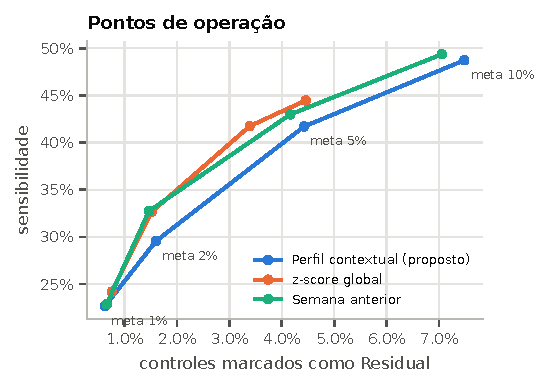
\includegraphics[width=0.85\columnwidth]{figuras/fig_curva_operacao.pdf}
  \caption{Curva de operação: sensibilidade contra controles marcados como \Residual, para metas de 1\%, 2\%, 5\% e 10\% de alarmes no histórico. A meta de 10\% coincide com o ponto adotado (percentil 97).}
  \label{fig:curva}
\end{figure}

\paragraph{Por motivo.} A sensibilidade depende fortemente do motivo (Figura~\ref{fig:sensmotivo}). Erros de sistema generalizados são detectados em 48\% a 89\% dos casos, conforme a intensidade, e erros 5xx de um consumidor em 51\% a 66\%. Erros de negócio têm detecção de 17\% a 48\% (generalizados) e de 24\% a 37\% (um consumidor), porque vários recursos já têm taxas altas e variáveis de 4xx. A latência vai de 11\% ($\times$1,5) a 59\% ($\times$4) e chega a \textbf{83\%} [79; 86] na degradação de 10 vezes.

\begin{figure}[t]
  \centering
  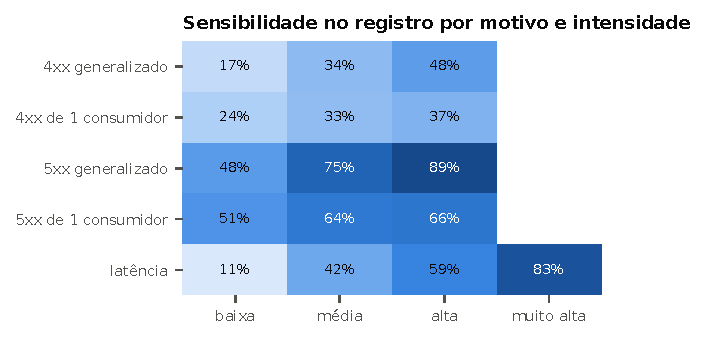
\includegraphics[width=0.9\columnwidth]{figuras/fig_sens_motivo.pdf}
  \caption{Sensibilidade no registro do método proposto, por motivo e intensidade.}
  \label{fig:sensmotivo}
\end{figure}

\paragraph{Por atraso do registro.} Como a decisão olha a hora inteira anterior ao registro, uma degradação que começou há pouco ocupa só parte dessa hora. Nas intensidades média e alta, a sensibilidade é de 42\% quando o incidente é registrado 15~min após o início da degradação, 55\% com 30~min e 59--62\% com 60 ou 120~min.

\paragraph{Por recurso e por mês.} Por recurso (Tabela~\ref{tab:recursos}), a sensibilidade vai de 7\% (E06) a 76\% (E05). Por mês, a sensibilidade foi de 60,3\% em agosto (7 recursos) e 42,0\% em setembro (12 recursos); restrita aos mesmos 7 recursos, setembro teve 58,8\%. A queda de setembro vem, portanto, sobretudo dos recursos que só entram nesse mês, com menos histórico e mais variação.

\subsection{Exp.~3: indicador responsável, início e abrangência}
Quando o recurso é sinalizado como \Residual, o indicador apontado é o do motivo injetado em 93,5\% dos casos [92,5; 94,3] (Figura~\ref{fig:confusao}): 96,8\% para 5xx generalizado, 95,6\% para 5xx de um consumidor, 94,0\% para latência e 87--88\% para 4xx. Os erros mais comuns são 4xx injetados apontados como volume ou latência (5\% a 7\% dos casos cada). A acurácia é menor em E06 (78\%) e E04 (87\%), recursos com muita variação natural em outros indicadores.

\begin{figure}[t]
  \centering
  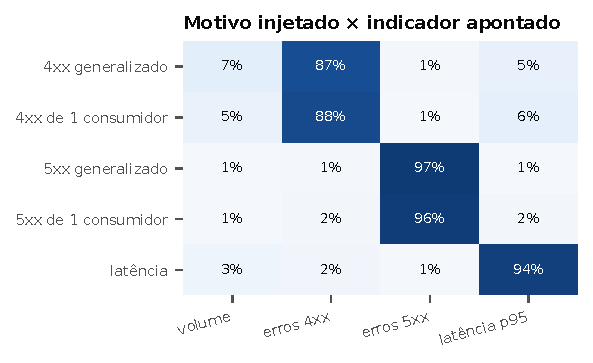
\includegraphics[width=0.85\columnwidth]{figuras/fig_confusao_indicador.pdf}
  \caption{Motivo injetado contra indicador apontado (casos detectados).}
  \label{fig:confusao}
\end{figure}

A Figura~\ref{fig:expansao} ilustra a expansão retroativa em um cenário de 5xx generalizado iniciado 60~min antes do registro. As três faixas mais recentes são residuais (2,5 a 3,1 vezes o limite) e a de 60--120~min é normal; o início é estimado entre 30 e 120~min antes do registro e contém o início real. Nos casos detectados, o início real ficou dentro da zona estimada em 89,4\% [88,2; 90,4] (Tabela~\ref{tab:consulta}): 93\% e 95\% quando a degradação começou 15 ou 30~min antes do registro, 87\% com 60~min e 85\% com 120~min (Figura~\ref{fig:inicio}). Em 1,4\% dos casos detectados na hora anterior, nenhuma faixa curta saiu do normal e o início fica indeterminado. Os demais erros são, na maioria, subestimações: uma faixa intermediária sai \Normal, a busca para cedo e o início é estimado mais perto do registro do que de fato ocorreu.

\begin{figure*}[t]
  \centering
  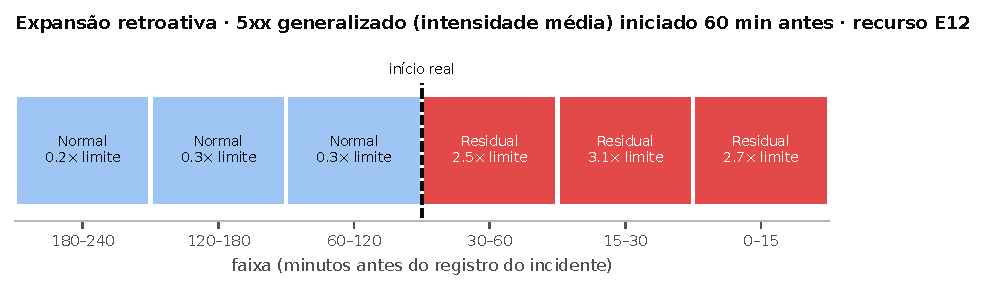
\includegraphics[width=0.85\textwidth]{figuras/fig_expansao_exemplo.pdf}
  \caption{Expansão retroativa em um cenário de 5xx generalizado iniciado 60~min antes do registro (E12): as três faixas mais recentes são residuais e a de 60--120~min é normal, e o início é estimado entre 30 e 120~min antes.}
  \label{fig:expansao}
\end{figure*}

\begin{figure}[t]
  \centering
  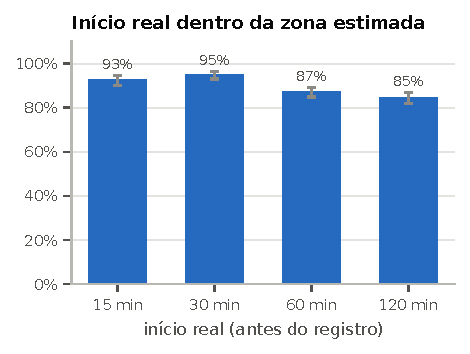
\includegraphics[width=0.8\columnwidth]{figuras/fig_inicio.pdf}
  \caption{Início real dentro da zona estimada, por atraso entre o início da degradação e o registro (IC de Wilson a 95\%).}
  \label{fig:inicio}
\end{figure}

\paragraph{Abrangência (complementar).} Entre os erros 4xx e 5xx detectados com o indicador correto, a abrangência foi classificada corretamente em 84,2\% [82,6; 85,7]. Os erros generalizados são reconhecidos como tais em 96--98\% dos casos; os de um consumidor, em 67\% (4xx) e 72\% (5xx). A hora inteira reúne mais requisições por cliente, o que torna a concentração dos erros mais fácil de medir.

\begin{table}[t]
  \caption{Exp.~3: qualidade da consulta nos incidentes detectados (método proposto, histórico de 3 meses), em \% (IC de Wilson a 95\%).}
  \label{tab:consulta}
  \small
  \begin{tabular}{lcc}
    \toprule
    Informação & Casos & Acerto \\
    \midrule
    Indicador responsável & 2.961 & 93,5 [92,5; 94,3] \\
    Início na zona estimada & 2.961 & 89,4 [88,2; 90,4] \\
    \quad degradação 15 ou 30~min antes & 1.264 & 93,9 \\
    \quad degradação 60 ou 120~min antes & 1.697 & 86,0 \\
    Abrangência (4xx e 5xx) & 2.073 & 84,2 [82,6; 85,7] \\
    \bottomrule
  \end{tabular}
\end{table}

\paragraph{Saída para o agente.} A consulta produz um documento estruturado. A Figura~\ref{fig:json} mostra, resumida, a saída do cenário da Figura~\ref{fig:expansao}.

\begin{figure}[t]
\begin{Verbatim}[fontsize=\scriptsize,frame=single]
{"recurso": "E12", "registro_incidente": "2026-08-02 16:52",
 "periodo_decisao": "02/08 15:52 a 16:52",
 "contexto": {"tipo_dia": "não útil", "hora": "16h"},
 "estado": "Residual", "indicador_impactado": "erros 5xx",
 "evidencias": [{"indicador": "erros 5xx", "observado": "16.2%",
    "faixa_normal_p5_p95": ["0.0%", "1.7%"], "vezes_o_limite": 3.59}],
 "inicio_estimado": "entre 30 e 120 min antes do registro",
 "abrangencia": {"classificacao": "generalizado",
    "clientes_ativos": 36, "clientes_com_erro": 17},
 "motivo_estatistico": "O recurso E12 está fora do regime normal
   esperado para não útil às 16h. Indicador impactado: erros 5xx
   — 16.2% na hora anterior ao registro (faixa normal 0.0% a
   1.7%), 3.59× o limite do recurso. O desvio começou entre 30 e
   120 min antes do registro. Os erros aparecem em 17 de 36
   consumidores ativos."}
\end{Verbatim}
\caption{Saída da consulta para o agente (resumida).}
\label{fig:json}
\end{figure}

\paragraph{Evento real.} Nos dados reais, sem injeção, a consulta para o E02 às 01h45 de 02/09 retornou \Residual por erros 5xx: 29,0\% na hora anterior ao registro (faixa normal de 0 a 1,1\% para dia útil à 1h), em 27 dos 31 consumidores ativos. O E02 tem um regime normal com 5xx elevado \emph{à 0h}; a hora avaliada (00h45 a 01h45) inclui o fim desse lote, o que eleva a taxa observada, mas os erros continuam nos 15~min finais (4,1\%), fora do horário do lote. A expansão retroativa estima o início entre 0 e 30~min antes do registro. O evento é um candidato a incidente real, a confirmar com a operação.

\subsection{Exp.~4: histórico de 3 meses $\times$ 1 mês}
Os dois históricos produziram resultados equivalentes no conjunto (Tabela~\ref{tab:historico}, Figura~\ref{fig:historico}): 48,7\% de sensibilidade e 92,5\% de especificidade com 3 meses, contra 49,1\% e 91,5\% com 1 mês (McNemar: $p=0{,}21$). O efeito, porém, difere por mês: em agosto, o histórico de 3 meses detectou mais (60,3\% contra 54,2\%), com especificidade igual; em setembro, o de 1 mês detectou mais (46,1\% contra 42,0\%), com especificidade um pouco menor (92,8\% contra 94,5\%). Os limites refletem a mudança de comportamento entre os meses: com 3 meses, o limite de 4xx do E09 fica 3,1 vezes maior e o de latência do E02, 2,8 vezes; já o limite de volume fica, na mediana, 24\% menor.

\begin{table}[t]
  \caption{Exp.~4: histórico de 3 meses $\times$ 1 mês (método proposto, em \%; m/a = intensidades média e alta).}
  \label{tab:historico}
  \small
  \begin{tabular}{lcccc}
    \toprule
    Histórico & Sensib. & Sensib. m/a & Especif. & Acur. indicador \\
    \midrule
    3 meses & 48,7 & 54,6 & 92,5 & 93,5 \\
    1 mês & 49,1 & 54,2 & 91,5 & 91,7 \\
    \bottomrule
  \end{tabular}
\end{table}

\begin{figure*}[t]
  \centering
  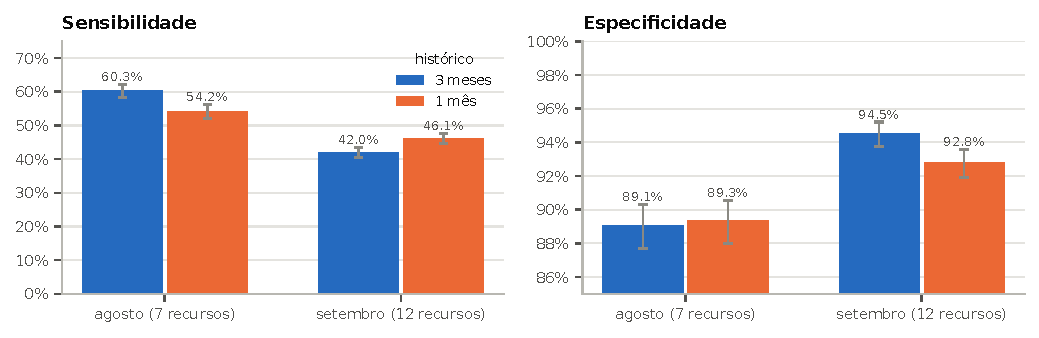
\includegraphics[width=0.85\textwidth]{figuras/fig_historico.pdf}
  \caption{Sensibilidade e especificidade por mês de teste e histórico, com IC de Wilson a 95\%.}
  \label{fig:historico}
\end{figure*}

\subsection{Critérios de sucesso}
Três dos cinco critérios definidos no entendimento do negócio foram atendidos (Tabela~\ref{tab:criterios}): a acurácia do indicador, o acerto do início e a ausência de perda para os baselines. A especificidade ficou pouco abaixo da meta, como efeito do ponto de operação escolhido, e a sensibilidade ficou abaixo da meta.

\begin{table}[t]
  \caption{Critérios de sucesso definidos antes da modelagem (hora anterior ao registro, histórico de 3 meses).}
  \label{tab:criterios}
  \small
  \begin{tabular}{p{0.5\columnwidth}p{0.22\columnwidth}c}
    \toprule
    Critério & Resultado & Atendido \\
    \midrule
    Controles com saída \Normal $\geq$ 95\% & 92,5\% & não \\
    Sensibilidade (média/alta) $\geq$ 70\% & 54,6\% & não \\
    Acurácia do indicador $\geq$ 90\% & 93,5\% & sim \\
    Início real na zona estimada $\geq$ 70\% & 89,4\% & sim \\
    Sem perda significativa para os baselines & sem perda & sim \\
    \bottomrule
  \end{tabular}
\end{table}

%% =====================================================================
\section{Discussão}\label{sec:discussao}

\paragraph{RQ1: regimes e estado no registro.} Os AALs agregados mostram regimes claros e ligados ao contexto em todos os recursos, sobretudo à hora do dia: lotes na virada do dia e à tarde, horário comercial em dias úteis, madrugada e até regimes normais com erros elevados em horários específicos. O perfil contextual representa esses múltiplos regimes diretamente: cada recurso tem 48 regimes normais de referência, um por tipo de dia e hora, cada um com a sua faixa normal, e o lote da meia-noite não é confundido com uma falha. Com a decisão sobre a hora anterior ao registro, o perfil supera um perfil sem contexto (z-score global) e empata com a semana anterior. Sua contribuição mais clara é a \emph{explicação}: a faixa normal do contexto e o limite de cada indicador são o que permite dizer ao operador ``16,2\% de 5xx às 16h de um dia não útil, quando o normal é até 1,7\%''. Para o operador, um resultado \Residual vem com o indicador certo e uma estimativa de início; um resultado \Normal indica que o recurso dificilmente é a origem, mas não descarta degradações sutis.

\paragraph{O limite por indicador.} A principal decisão de modelagem foi normalizar cada indicador pela sua própria cauda no recurso. Sem isso, os indicadores com picos reais frequentes (taxas de 4xx em E04 e E07) definem o limiar e escondem desvios de latência e de erros de sistema. Esse achado é, por si, relevante para a prática: em AALs reais, os indicadores não têm a mesma variabilidade, e um único limiar global sobre todos eles tende a privilegiar os mais ruidosos.

\paragraph{RQ2: indicador e início.} O ponto mais forte do método é a qualidade da informação quando ela é emitida: o indicador responsável é apontado corretamente em 94\% dos casos, e o início é localizado na zona certa em 89\%. A separação de papéis é simples de explicar: a hora anterior decide \emph{se} há desvio, comparada ao regime do contexto, e as faixas curtas da expansão retroativa dizem \emph{desde quando}, olhando para trás até encontrar um período normal. A zona estimada é estreita quando o desvio é recente (0--30 ou 15--60~min) e mais larga quando ele é antigo, o que corresponde à precisão de que o operador precisa em cada caso.

\paragraph{Decisão por hora.} A janela de 1~h é coerente com os regimes, que são horários, e dá estimativas estáveis: a abrangência, por exemplo, acerta 84\%. O custo aparece nos incidentes registrados logo após o início da degradação: com 15~min de atraso, só um quarto da hora avaliada está degradado, e a sensibilidade cai para 42\%. A janela é deslizante e pode atravessar a fronteira de dois contextos, como no evento real do E02, em que a hora avaliada incluiu o fim do lote da meia-noite.

\paragraph{Ponto de operação.} O percentil 97 equilibra detecção e alarmes: cerca de metade dos incidentes é sinalizada, e 7,5\% dos controles saem como \Residual. Como a consulta só é feita quando já existe um incidente aberto, um falso \Residual custa uma verificação a mais para o operador, e não um alarme fora de hora. Se o custo dessa verificação for alto, a curva de operação mostra pontos mais conservadores.

\paragraph{RQ3: quanto histórico.} Mais histórico não significou um perfil melhor: os dois históricos empatam no conjunto, e cada um ganha em um mês. As APIs mudam de patamar ao longo dos meses (volume crescendo, taxas de erro de negócio mudando), e um histórico de três meses inclui comportamentos que podem já não valer, o que alarga ou desloca os limites. Para a implantação, isso favorece o \emph{retreino mensal}, e o histórico de 1 mês, mais simples de manter, é suficiente.

\paragraph{Por que a latência e os erros de negócio são pouco sensíveis.} O p95 das médias por minuto tem caudas pesadas mesmo em dias normais (0,78\% das horas passam de 10 vezes a mediana do contexto), o que obriga limites altos: a latência é detectada em 83\% dos casos com a degradação de 10 vezes e em 59\% com 4 vezes, mas pouco nas degradações moderadas. Um percentil por requisição, se disponível no gateway, é o caminho natural de melhoria. Com os erros de negócio ocorre o mesmo: recursos com picos reais frequentes de 4xx (E04, E07) recebem limites altos para esse indicador, e só desvios grandes aparecem. Em E06, com muitos clientes e variação natural alta, a sensibilidade foi de 7\%. Nesses casos, o próprio limite é uma informação útil: ele diz ao operador que aquele indicador já é instável no recurso.

%% =====================================================================
\section{Ameaças à validade}\label{sec:ameacas}

\paragraph{Falhas sintéticas.} O desempenho mede a capacidade de detectar \emph{os motivos injetados}, e não falhas reais. As intensidades variadas, os quatro atrasos, os dois meses e o grande número de cenários reduzem, mas não eliminam, esse viés. A acurácia do indicador, do início e da abrangência é medida apenas sobre incidentes detectados, que tendem a ser os mais fortes.

\paragraph{Parâmetros do método.} O percentil 97, a decisão sobre a hora anterior ao registro e a intensidade de latência $\times$10 foram fixados sem otimização nos cenários de teste. A intensidade $\times$10 é justificada pela distribuição do histórico, e as intensidades menores são relatadas. No k-means, os indicadores foram limitados aos percentis 1 e 99 para que picos isolados não formassem grupos triviais; como o k-means é descritivo, isso não afeta as métricas de decisão.

\paragraph{Janela deslizante e contexto.} A hora anterior ao registro raramente coincide com uma hora cheia, e o seu contexto é dado pela hora do ponto médio da janela. Perto de mudanças bruscas de regime, como o início ou o fim de um lote, a janela mistura dois contextos.

\paragraph{Controles e anomalias reais.} As consultas de controle usam dados reais sem injeção, que podem conter anomalias reais (como a do E02), contadas como falso \Residual. A especificidade é, portanto, uma estimativa conservadora.

\paragraph{Cobertura desigual.} Cinco recursos só têm dados a partir de 16/07 e entram apenas no teste de setembro, quatro deles até 03/09; nesses, o ``histórico de 3 meses'' tem na prática cerca de seis semanas. Os feriados considerados foram 01/05, 04/06 (Corpus Christi, tratado como não útil) e 07/09.

\paragraph{Latência aproximada.} O p95 é calculado sobre as médias por minuto e por cliente, e não sobre requisições; a cauda real tende a ser maior. Uma latência 10 vezes maior poderia, na prática, esbarrar no \emph{timeout} do gateway e virar erro 504, o que a injeção não simula.

\paragraph{Generalização.} Os resultados vêm de uma organização e de 12 recursos. A base não pode ser compartilhada; o código dos notebooks é independente dos dados.

%% =====================================================================
\section{Considerações finais}\label{sec:conclusao}

Este trabalho mostrou que Access Logs agregados por minuto, sem \emph{traces} nem logs de aplicação, permitem caracterizar os múltiplos regimes normais de cada recurso de API, um por tipo de dia e hora, e informar, no instante em que um incidente é aberto, se a hora anterior ao registro está dentro do regime normal do seu contexto e, se não, qual indicador foi impactado (erros de negócio, erros de sistema ou latência) e desde quando. O método usa técnicas simples (mediana, MAD, percentis, validação cruzada e uma busca retroativa), não exige rótulos e produz uma explicação que um agente ou operador pode usar diretamente.

Em dois meses de teste, a informação foi confiável quando emitida: 93,5\% de acerto no indicador e 89,4\% de acerto na zona de início, com 92,5\% de especificidade. A sensibilidade foi de 49\%: alta para erros de sistema e para degradações grandes de latência, e baixa para erros de negócio em recursos com muitos 4xx naturais. O perfil contextual superou um perfil sem contexto e empatou com a comparação com a semana anterior; seu valor maior está na explicação. Os históricos de 3 meses e de 1 mês se equivaleram, o que recomenda retreino mensal com o histórico recente.

Como trabalhos futuros, destacam-se: (i) validar o método com incidentes reais, começando pelo evento observado no E02, e com a avaliação de operadores; (ii) testar históricos deslizantes com pesos maiores para o período recente; (iii) tratar a janela que atravessa dois contextos, ponderando o regime de cada hora pela sua parte na janela; (iv) melhorar a sensibilidade à latência com percentis por requisição; e (v) integrar a consulta como ferramenta de um agente de apoio a incidentes.

\bibliographystyle{ACM-Reference-Format}
\bibliography{referencias}

\end{document}
